The Heavy Truck Cape with BeagleBone is a versatile Linux device designed for use with heavy vehicles. It has the ability to interface with different vehicle communication protocols both in and outside of userspace. This guide is designed to inform the reader over the many features of the device, as well as how to build your own tools.

\begin{figure}[h]
    \centering
    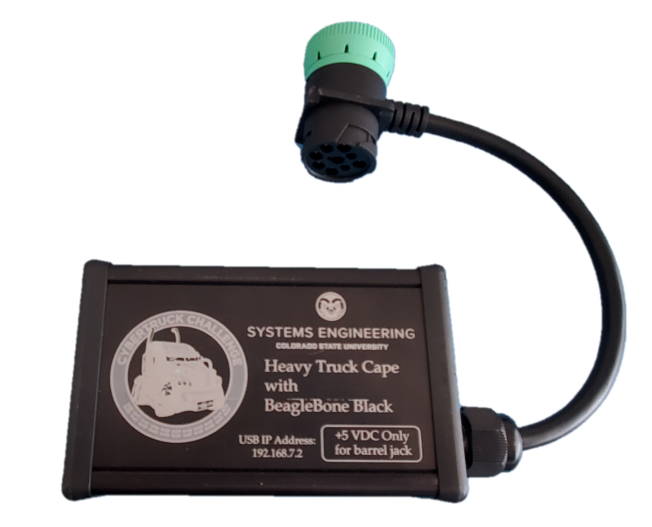
\includegraphics[width=0.5\textwidth]{images/beagleboneblack_truckcape_v4_images/BeagleboneTC.png}
    \caption{Heavy Truck Cape w/ Beaglebone Black}
    \label{fig:Beaglebone Black}
\end{figure}


\section{Device Hardware}
    The Heavy Vehicle Truck Cape device is made up of two primary components: the BeagleBone Black and the Truck Cape. The cape provides additional peripheral connections for the BeagleBone. The BeagleBone is a Linux microcomputer with two on-board microcontrollers called ``Programmable Realtime Units" (PRUs).

    \subsection{BeagleBone Black}
        The \href{https://beagleboard.org/black}{BeagleBone Black} is a Linux Microcomputer. It is called a ``microcomputer" because it is a feature complete computer small enough to fit in the palm of your hand. With an on-board USB port and a micro-HDMI connector, one could connect the BeagleBone to a monitor and a keyboard for a ``full" computer experience. 

    \subsection{Truck Cape}
        The Heavy Vehicle Truck Cape provides more interface connections for the BeagleBone as well as power delivery for the components on the cape. 

        \begin{figure}
            \centering
            \begin{minipage}[b]{0.4\textwidth}
                \includegraphics[width=\textwidth]{images/beagleboneblack_truckcape_v4_images/TC-NoBBB.png}
                \caption{Truck Cape Board w/o BeagleBone.}
            \end{minipage}
            \hfill
            \begin{minipage}[b]{0.4\textwidth}
                \includegraphics[width=\textwidth]{images/beagleboneblack_truckcape_v4_images/TC-BBB.png}
                \caption{Truck Cape Board w/ BeagleBone Installed.}
            \end{minipage}
        \end{figure}

        As shown in figure 2 and figure 3, the BeagleBone is installed directly onto the cape board. It is then placed inside of an enclosure (fig. 1). Very little logic is performed on the cape. Its primary function is to provide peripheral interfaces for the BeagleBone to use. The logic performed by the cape is relegated to lower-level connection logic for CAN and other vehicle communication standards. 

    \subsection{Device Connections}

    \subsection{Future Work}
        Future work may include the installation of a newer form of BeagleBone, such as the BeagleBone Black Wireless.  The current iteration of the Truck Cape has a few design flaws which must be fixed manually at the end of production. Future work may also include a new Truck Cape schematic without these design artifacts and with surface-mounted components.

    \subsection{Device Assembly}
    This section may be out of date (January 2021). It is written for the v4 hardware. The most detailed and up-to-date guide to assemble the device may be found on the \href{https://github.com/SystemsCyber/TruckCapeProjects}{Truck Cape Projects GitHub Repository.}
        \subsubsection{PCB Assembly}
        \subsubsection{Hardware Errata}
            This section is unique to the v4 version of the hardware. 
        \subsubsection{BeagleBone Truck Cape Assembly}
        \subsubsection{Laser Etching and Cutting the Enclosure}
        \subsubsection{Deutch 9 Pin to Molex Connector for Enclosure}
        \subsubsection{Enclosure Assembly}

\section{Device Firmware}
    All firmware is located on the BeagleBone. As mentioned earlier, the truck cape has very litinternal logic. The logic performed by the cape is performed on prefabricated microchips suchthe MCP 2562 CAN Controller. Although one could install any number of different operating systand device firmwares, this guide will focus on the image and software used by the Systems CyProgram at Colorado State Universi
    \subsection{BootLoader}
        A bootloader is a low-level software which is used to install firmware onto an embeddevice. The BeagleBone Black uses u-boot for its bootloader. However, the easiest wayprogram the BeagleBone firmware is to create a flashable SD Car
    \subsection{Operating System}
        While varying operating systems may be installed on the BeagleBone, the chosen operatsystem for this guide is a flavor of Debian Linux. The most detailed and up-to-date guideconfigure the operating system may be found on the \href{https://github.com/SystemsCyTruckCapeProjects}{Truck Cape Projects GitHub Repository.}
    \subsection{Future Work}
        There are many ways to flash software onto the BeagleBone, including some which are possithrough remote access. Future work may include a toolchain for the remote reprogrammingHeavy Vehicle Truck Cape Devices. 
\section{Embedded Linux Operating System: Installation, Basic Use, and Configuration}
    This portion of the guide covers the initial installation and configuration of the Linux operating system. This guide may be out of date (January 2021), so refer to the \href{https://github.com/SystemsCyber/TruckCapeProjects}{Truck Cape Projects GitHub Repository} for the most up-to-date installation instructions.
    
    If you already have a fully configured BeagleBone, you may skip ahead to PC Necessary Software.

    \subsection{Base Installation}
        The Linux image to run on the BeagleBone's eMMC can be downloaded, decompressed, imaged to an SD card. When the BeagleBone Black boots from the SD card, it will burn the eMMC to have the necessary contents to run the exercises in this repository. 

        For the impatient, here is a link to the most current image based on the modifications: \href{https://www.engr.colostate.edu/~jdaily/files/TruckCapeImage-2020-11-14_4.19.img.xz}{TruckCapeImage-2020-11-14\_g.xz}
        
        To start from scratch, here is a link to the chosen Linux base image:  \href{https://debian.beagleboard.org/images/bone-eMMC-flasher-debian-10.3-iot-armhf-2020-04-06-4gb.img.xz}{bone-eMMC-flasher-debian-10.3-iot-armhf-2020-04-06-4gb.img.xz}
        
        \subsubsection{Installing the Linux Image via SD Card Flasher Image}
            This process is the same if you are starting from the pre-built image or from scratch.
            
            \begin{enumerate}
                \item Download your chosen image file (pre-built or scratch)
                \item Using a compression utility such as \href{https://www.7-zip.org/}{7-Zip} or \href{https://www.win-rar.com/start.html?&L=0}{WinRAR} decompress the image
                \item Using a program like \href{https://win32diskimager.org/}{Win32DiskImager} or \href{https://www.balena.io/etcher/}{Balena Etcher} burn the image file onto a 4 GB SD Card.
                \item Disconnect power from the BeagleBone, then insert the SD card into the SD card slot on the back of the BeagleBone. 
                \item While holding down the button near the USB Port (Red Circle in Fig. \ref{fig:BeagleBoneButtonLED}), Power On the BeagleBone. Continue holding the button until all four of the User LEDs (Blue Rectangle in Fig. \ref{fig:BeagleBoneButtonLED}) turn on. Once all four are lit, release the button.
                    \begin{figure}[H]
                        \centering
                        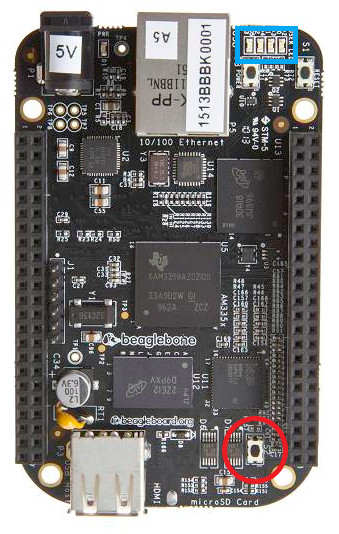
\includegraphics[width=0.5\textwidth]{images/beagleboneblack_truckcape_v4_images/BeagleBoneFormatButton.png}
                        \caption{BeagleBone Format Button (Red Circle) and User LEDs (Blue Rectangle)}
                        \label{fig:BeagleBoneButtonLED}
                    \end{figure}
                \item The LEDs will then flash intermittenly for a few seconds before assuming a back-and-forth pattern. This process takes some time, up to ten or even fifteen minutes. Eventually, the pattern will stop, all LEDs will light up before turning off. 
                \item Once all of the LEDs are off, disconnect power, remove the SD card from the slot, and power on the BeagleBone. The first boot may take longer than others. 
                \item You may now connect to the BeagleBone
            \end{enumerate}
        \subsubsection{Building and Installing Linux Kernel from Scratch}
        
    \subsection{PC Necessary Software}
        These Linux images do not have the video output enabled. They are designed for a host device (PC) to log in to the terminal of the BeagleBone. If this is your first time with a Heavy Truck Cape with BeagleBoneBlack, then you'll need some software on your computer to interface with it. 
        
        \subsubsection{Windows Software}
        Windows users will need the following:
            \begin{enumerate}
                \item SSH Software: \href{https://www.chiark.greenend.org.uk/~sgtatham/putty/}{PuTTY}
                \item SCP Software: \href{https://winscp.net/eng/index.php}{WinSCP}  or \href{https://filezilla-project.org/}{FileZilla}
            \end{enumerate}
        \subsubsection{Linux Software}
        Linux users will need the following:
            \begin{enumerate}
                \item SSH Software: \href{https://linuxcommandlibrary.com/man/ssh}{SSH}
                \item SCP Software: \href{https://linuxcommandlibrary.com/man/scp}{SCP}
            \end{enumerate}
        \subsubsection{Mac Software}
        Mac users will need the following terminal commands:
        \begin{enumerate}
                \item SSH Software: SSH
                \item SCP Software: SCP
            \end{enumerate}
        
    \subsection{Remote Connecting to the Beaglebone}
        

        \subsubsection{Logging into Terminal through USB with Putty}

            \begin{enumerate}
                \item Plug in the a Mini USB cable between the BeagleBone and your computer
                \item Give the system some time to boot. This may take several minutes. In Windows, the BeagleBone should appear in File Explorer when ready.
                \item Open PuTTY
                \item Specify the Host Name (or IP address) as 192.168.7.2 and port 22 (Fig. \ref{fig:PuTTY Window}). 
                    \begin{figure}[H]
                        \centering
                        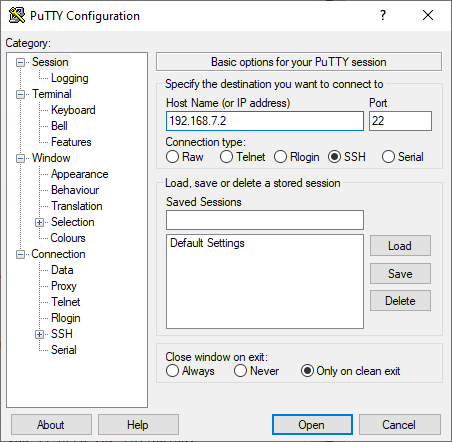
\includegraphics[width=0.5\textwidth]{images/beagleboneblack_truckcape_v4_images/PuttyWindow.png}
                        \caption{PuTTY Window}
                        \label{fig:PuTTY Window}
                    \end{figure}
                \item (Optional) For easier access in the future, the session access information may be saved in PuTTY. Write \textless username\textgreater@\textless ipaddress\textgreater  in the "Saved Sessions" field. For this guide, the session is "debian@192.168.7.2" (Fig. \ref{fig:PuTTYSavedSession}). Then click "save"
                \begin{figure}[h]
                    \centering
                    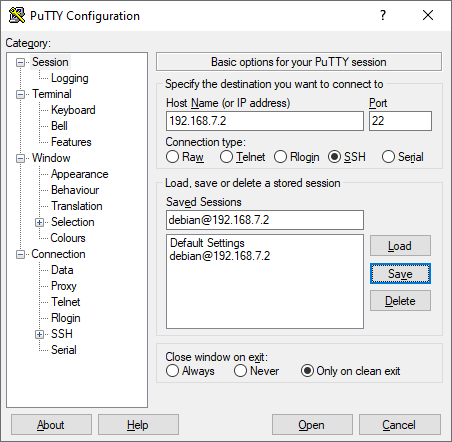
\includegraphics[width=0.5\textwidth]{images/beagleboneblack_truckcape_v4_images/PuttySavedSession.png}
                    \caption{PuTTY Saved Session}
                    \label{fig:PuTTYSavedSession}
                \end{figure}
                \item Press Open
                \item Enter the login credentials: 
    
                Default Credentials U: debian P: temppwd 
    
                (If connected to the internet, this password should be changed).
                
                If the password has been changed from the default, contact an administrator for access.
    
                There may be a warning about the security of the device. This is in reference to the SSH certificate offered by the device. This may be accepted.
    
                \item PuTTY should now be logged into the Debian account on the BeagleBone. A Window should open similar to Fig. \ref{fig:OpenSession}. 
                    \begin{figure}[H]
                        \centering
                        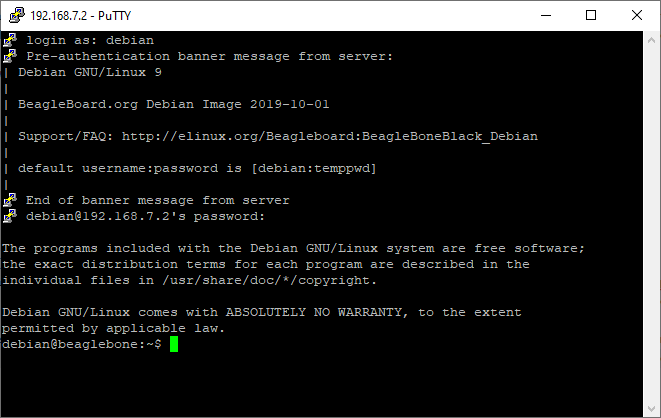
\includegraphics[width=0.5\textwidth]{images/beagleboneblack_truckcape_v4_images/PuttySession.png}
                        \caption{Open Session}
                        \label{fig:OpenSession}
                    \end{figure}
            \end{enumerate}
        
        \subsubsection{Logging into Terminal through USB with SSH (Linux and Mac)}
        
        \subsection{File Transfer between Computer and BeagleBone}
        The easiest way to copy and move files between a Windows computer and a BeagleBone is through an SCP software like WinSCP or FileZilla.
            \subsubsection{File Transfer with WinSCP}
            WinSCP is an SCP program available for Windows.
            \begin{enumerate}
                \item Set the BeagleBone as if starting an SSH connection. Either ensure that the BeagleBone is fully connected via USB or is powered and connected to the network.
                \item Start WinSCP on the Windows Computer
                \item Enter BeagleBone access credentials. This process is very similar to starting a PuTTY connection (Fig. \ref{fig:WinSCPCredentials})
                \begin{figure}[H]
                    \centering
                    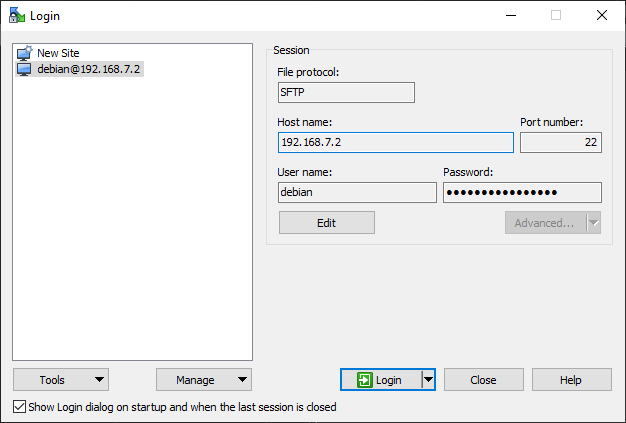
\includegraphics[width=0.5\textwidth]{images/beagleboneblack_truckcape_v4_images/WinSCPcredentials.png}
                    \caption{WinSCP Credentials Menu}
                    \label{fig:WinSCPCredentials}
                \end{figure}
                \item Optional: If desired, save the credentials for quick future access.
                \item There may be some popups about the security of the connection. This is due to how the BeagleBone handles certificates. They may be accepted.
                \item If the connection is successful, a dual-explorer window will open. The left pane is the Windows Computer file system, the right pane is the BeagleBone file system. You may navigate the two file systems and move/copy files.
                \item When finished, close the window.
            \end{enumerate}
            \subsubsection{File Transfer with FileZilla}
            \begin{enumerate}
                \item Set the BeagleBone as if starting an SSH connection. Either ensure that the BeagleBone is fully connected via USB or is powered and connected to the network.
                \item Start FileZilla on the Windows Computer
                \item Enter BeagleBone access credentials at the top of the window. This process is very similar to starting a PuTTY connection (Fig. \ref{fig:FileZillaCredentials}).
                \begin{figure}[H]
                    \centering
                    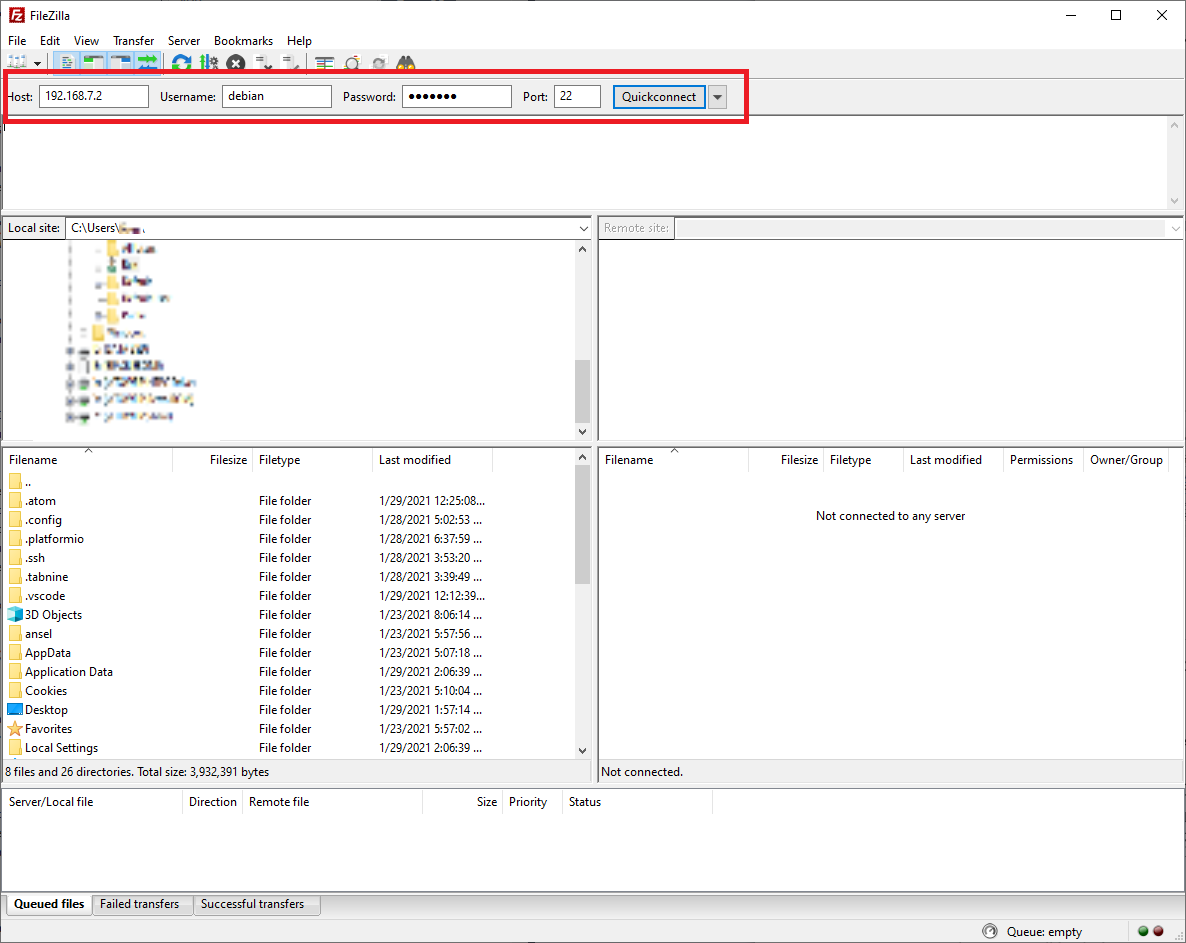
\includegraphics[width=0.5\textwidth]{images/beagleboneblack_truckcape_v4_images/FileZillaCredentials.png}
                    \caption{FileZilla Credentials Menu}
                    \label{fig:FileZillaCredentials}
                \end{figure}
                \item Optional: If desired, save the credentials for quick future access.
                \item There may be some popups about the security of the connection. This is due to how the BeagleBone handles certificates. They may be accepted.
                \item If the connection is successful, a dual-explorer window will open. The left pane is the Windows Computer file system, the right pane is the BeagleBone file system. You may navigate the two file systems and move/copy files.
                \item When finished, close the window.
            \end{enumerate}

            \subsubsection{SCP File Transfer between Linux/Mac and BeagleBone}
        
            \subsubsection{Logging in through Ethernet}
                If the BeagleBone is instead powered externally and connected via Ethernet, follow the same instructions as logging in through USB, except use the Ethernet IP address of the BeagleBone for the Host Address. 
    \subsection{Linux Basics}
        This guide is not designed to replace other Linux how-to guides and tutorials. The internet wbe the     best resource for Linux information. It is important to have a basic understanding of Linux Operating   System. In Linux, everything is a file. Directories (read "folders" for Windusers) are files which    point to other files. Linux allows near-total control of the OperatSystem. Unlike Windows where    certain files or folders are protected from users, Linux trusts tthe user knows best and allows them   to execute whatever they like assuming they have the proprivileges. 
        
        Privileges are separated into user, group, and everyone. 
        
        A Linux "root" user is a user with unlimited privileges. Root accounts are generally locked dto     prevent unauthorized access. Because of this, Linux configurations usually include a "suusers" group    which provides limited root access for users. This is useful so that files importto the operating  system are not accidentally modified or deleted though users may still modifydelete these files if   they login as root.
        \subsubsection{Basic Linux Commands}
            Particularly useful basic commands are listed below.
            \begin{table} 
                \begin{tabularx}{\textwidth}{X*{5}{>{\centering\arraybackslash}X}} 
                    \hline
                    Command & Description \\
                    \hline \hline 
                    man \textless command\textgreater & Manual for Command  \\
                    \hline
                    ls & list everything in current directory \\
                    \hline
                    cd \textless directory\textgreater& change directory \\
                    \hline
                    sudo \textless command\textgreater & Execute command as "super user" \\
                    \hline
                    mkdir \textless newDirectory\textgreater & Make new Directory \\
                    \hline
                    chmod \textless file\textgreater  \textless accessCode\textgreater & Change access      permissions of file \\
                    \hline
                    mv \textless sourcefile\textgreater  \textless destination\textgreater & move (or   rename)   file \\
                    \hline
                    cp \textless sourcefile\textgreater  \textless destination\textgreater & copy file \\
                    \hline
                    rm \textless file\textgreater & Remove file \\
                    \hline
                    rm -r \textless DIR\textgreater & Recursively delete all directories and files starting     from    DIR \\
                    \hline
                    nano \textless file\textgreater & text editor \\
                    \hline
                \end{tabularx} 
            \end{table}
            This list is by no means exhaustive, but should be enough to explore the file system and continue   with this guide. Sometimes commands must be used in conjunction with another command. For     instance, when trying to remove a directory, the user may need to type: 
            \begin{lstlisting}[language=bash, autogobble=true]
                sudo rm -r DirectoryToDelete
            \end{lstlisting}
            Also of note: Linux files and directories ARE case sensitive. The file "foo" is a different file than "Foo".
    \subsection{Configuring Linux}
        This portion of the guide will assume that you are starting from scratch.
        
        If you have a pre-configured BeagleBone, you may skip the remainder of this chapter.
        
        This portion of the guide also assumes that the BeagleBone is connected to the internet through the     ethernet port. It is possible to perform a full offline installation of the software by moving  packages to the BeagleBone over SCP. However, that is beyond the scope of this guide.
        
        \subsubsection{Testing the System}
            Using an SSH client, like PuTTY, and a USB to computer connection, connect to the Beagle Bone   Black SSH using IP 192.168.7.2 on port 22.
    
            The new login uses the following credentials:
    
            U: debian
    
            P: temppwd
    
            The availability if this connection may take longer than you might like, but be patient, the    board will finish booting and enumerate as a drive on your host computer. 
            Connect a live Internet connection by the Ethernet cable into your Beagle Bone Black. Check to  see if you have a valid IP address on `eth0`:
            
            \begin{lstlisting}[language=bash, autogobble=true]
                $ ifconfig
            \end{lstlisting}
                \subsubsection{Version Check}
                If you are having troubles, be sure you are using the same version that's documented here.  When the kernel changes, the results may be different. 
                
                Enter the following command to check the image version:
                \begin{lstlisting}[language=bash, autogobble=true]
                    debian@beaglebone:~$ cat /etc/dogtag
                    BeagleBoard.org Debian Buster IoT Image 2020-04-06
                \end{lstlisting}
                Enter the following command to check the kernel version:
                \begin{lstlisting}[language=bash, autogobble=true]
                    debian@beaglebone:~$ uname -a
                    Linux beaglebone 4.19.94-ti-r42 #1buster 
                    SMP PREEMPT Tue Mar 31 19:38:29 UTC 2020 armv7l GNU/Linux
                \end{lstlisting}
        \subsubsection{Disable Unused Hardware}
            Edit the uEnv.txt file and uncomment the some disable commands. This opens the pins up faccessing   other functions.
            \begin{lstlisting}[language=bash, autogobble=true]
                sudo nano /boot/uEnv.txt
            \end{lstlisting}
            Uncommment the disable\_uboot\_overlay as follows:
            \begin{lstlisting}[language=bash, autogobble=true]
                #dtb_overlay=/lib/firmware/<file8>.dtbo
                ###
                ###Disable auto loading of virtual capes (emmc/video/wireless/adc)
                #disable_uboot_overlay_emmc=1
                disable_uboot_overlay_video=1
                disable_uboot_overlay_audio=1
                disable_uboot_overlay_wireless=1
                disable_uboot_overlay_adc=1
                ###
            \end{lstlisting}
            Be sure to keep the emmc line commented, since that's the root file system.
    
            Also, enable the universal overlay. This ensures the kernel has access to the hardware  pmultiplexers. 
    
            \begin{lstlisting}[language=bash, autogobble=true]
                ###Additional custom capes
                uboot_overlay_addr4=/lib/firmware/cape-universal.dtbo
                #uboot_overlay_addr5=/lib/firmware/<file5>.dtbo
                #uboot_overlay_addr6=/lib/firmware/<file6>.dtbo
                #uboot_overlay_addr7=/lib/firmware/<file7>.dtbo
                ###
            \end{lstlisting}
    
            Finally, enable uio\_pruss kernel module for the Programmable Realtime Unit (PRU).
            \begin{lstlisting}[language=bash, autogobble=true]
                ###PRUSS OPTIONS
                ###pru_rproc (4.14.x-ti kernel)
                #uboot_overlay_pru=/lib/firmware/AM335X-PRU-RPROC-4-14-TI-00A0.dtbo
                ###pru_rproc (4.19.x-ti kernel)
                #uboot_overlay_pru=/lib/firmware/AM335X-PRU-RPROC-4-19-TI-00A0.dtbo
                ###pru_uio (4.14.x-ti, 4.19.x-ti & mainline/bone kernel)
                uboot_overlay_pru=/lib/firmware/AM335X-PRU-UIO-00A0.dtbo
                ###
            \end{lstlisting}
    
            Save and reboot: `sudo shutdown -r now`
    
            Verify the uio\_pruss kernel module is running:
            \begin{lstlisting}[language=bash, autogobble=true]
                lsmod | grep pru
            \end{lstlisting}

        \subsubsection{Setup Pin Multiplexing}
            Write the following commands to get the CAN hardware to access the pins upon boot. 
            Create a file in the /etc directory:
    
            \begin{lstlisting}[language=bash, autogobble=true]
                sudo nano /etc/pin_config.sh
            \end{lstlisting}
                Write the following into the directory:
            \begin{lstlisting}[language=bash, autogobble=true]
                #!/bin/sh -e
                # DCAN1
                config-pin p9.24 can
                config-pin p9.26 can 
                # DCAN0
                config-pin p9.19 can
                config-pin p9.20 can
                #ttyO2:
                config-pin p9.21 uart
                config-pin p9.22 uart
                #ttyO4:
                config-pin p9.11 uart
                config-pin p9.13 uart
                #ttyO5:
                config-pin p8.37 uart
                config-pin p8.38 uart
                # PWMs
                config-pin p8.46 pwm
                config-pin p8.45 pwm
                config-pin p8.34 pwm
                config-pin p8.36 pwm
                # GPIO
                config-pin p9.12 gpio
                config-pin p9.14 gpio
    
                exit 0
            \end{lstlisting}
            Make the script executable:
            \begin{lstlisting}[language=bash, autogobble=true]
                sudo chmod +x /etc/pin_config.sh
            \end{lstlisting}
            However, these commands need to be run upon boot, so let's make a script to do this and it to   a   boot sequence.
    
            \begin{lstlisting}[language=bash, autogobble=true]
                sudo nano /lib/systemd/system/pin_config.service
            \end{lstlisting}
            Add this to the file:
            \begin{lstlisting}[language=bash, autogobble=true]
                [Unit]
                Description=Setup for BBB
    
                [Service]
                Type=simple
                ExecStart=/bin/bash /etc/pin_config.sh
    
                [Install]
                WantedBy=multi-user.target
            \end{lstlisting}
    
            Start the service
    
            \begin{lstlisting}[language=bash, autogobble=true]
                sudo systemctl start pin_config.service
            \end{lstlisting}
            Verify the service
    
            \begin{lstlisting}[language=bash, autogobble=true]
                sudo systemctl status pin_config.service
            \end{lstlisting}
            Enable the service at boot
    
            \begin{lstlisting}[language=bash, autogobble=true]
                sudo systemctl enable pin_config.service
            \end{lstlisting}
            To confirm the pin\_config.service was enabled, look for a symbolic link in `/etc/systsystem`
    
            \begin{lstlisting}[language=bash, autogobble=true]
                debian@beaglebone:/etc/systemd/system$ ls -la
                lrwxrwxrwx  1 root root   38 Sep 17 04:51 pin_config.service -> /lib/systemd/system/    pin_config.service
            \end{lstlisting}
    
            Reboot and verify. `sudo shutdown -r now`
    
            \begin{lstlisting}[language=bash, autogobble=true]
                debian@beaglebone:~$ config-pin -q p9.24
    
                Current mode for P9_24 is:     can
    
            \end{lstlisting}
    
            Verify the status of the pin\_config.service was successful by looking for an output lthis:
    
            \begin{lstlisting}[language=bash, autogobble=true]
                debian@beaglebone:~$ sudo systemctl status pin_config.service
                pin_config.service - Setup for BBB p
                Loaded: loaded (/etc/systemd/system/pin_config.service; enabled; vendor preset: enabled)
                Active: inactive (dead) since Tue 2020-09-08 23:52:06 UTC; 2min 18s ago
                Process: 856 ExecStart=/bin/bash /home/debian/pin_config.sh (code=exited, statuSUCCESS)
                Main PID: 856 (code=exited, status=0/SUCCESS)
    
                Sep 21 14:06:18 beaglebone bash[2040]: Current mode for P9_13 is:     uart
                Sep 21 14:06:18 beaglebone bash[2040]: Current mode for P8_37 is:     uart
                Sep 21 14:06:18 beaglebone bash[2040]: Current mode for P8_38 is:     uart
                Sep 21 14:06:18 beaglebone bash[2040]: Current mode for P8_46 is:     pwm
                Sep 21 14:06:18 beaglebone bash[2040]: Current mode for P8_45 is:     pwm
                Sep 21 14:06:18 beaglebone bash[2040]: Current mode for P8_34 is:     pwm
                Sep 21 14:06:18 beaglebone bash[2040]: Current mode for P8_36 is:     pwm
                Sep 21 14:06:18 beaglebone bash[2040]: Current mode for P9_12 is:     gpio
                Sep 21 14:06:18 beaglebone bash[2040]: Current mode for P9_14 is:     gpio
                Sep 21 14:06:18 beaglebone systemd[1]: pin_config.service: Succeeded.
            \end{lstlisting}
            If this doesn't work, be sure to disable the overlays in the uEnv.txt file.
        
        \subsubsection{Network Interface Configuration}   
        \subsubsection{Add Virtual CAN Drivers}
            
        \subsubsection{Additional Software and Drivers}
        \subsubsection{Truck Cape Projects}
            
        \subsubsection{J1708 Drivers}
            
        \subsubsection{Writing Current Linux Image to SD Card}    
\section{CAN on BeagleBone}
    \subsection{CAN Channels}
        The BeagleBone is generally configured to have multiple CAN Channels. Usually, these channels are can0, can1, vcan0, and vcan1. VCan is a "virtual CAN bus" that to the BeagleBone appears to be a normal CAN channel. However, this CAN channel does not send messages on any physical bus. Only the BeagleBone hosting the virtual CAN network can send or receive messages. Because of this "loopback" functionality, the virual CAN channels are often used for device and application testing.
        \subsubsection{Baudrate}
            The term baudrate is generally interchangeable with the term bitrate. Either way, it refers to the speed of the bus in bits-per-second. The BeagleBone uses 250k baud (250,000 bits per second) by default. To set the baudrate, use the following commands, replacing \textless channel\textgreater with the channel name and \textless baudrate\textgreater  with the desired baudrate (usually 125kbps, 250kbps, 500kbps, or 1000kbps). Below is the general syntax for changing the baudrate of a CAN channel on the BeagleBone. If you are having connectivity issues, you may have the channel set at the incorrect baudrate.
            \begin{lstlisting}[language=bash, autogobble=true]
                $ sudo ip link set <channel> down
                $ sudo ip link set <channel> up type can bitrate <baudrate>
            \end{lstlisting}
            An example is shown below
            \begin{lstlisting}[language=bash, autogobble=true]
                $ sudo ip link set can0 down
                $ sudo ip link set can0 up type can bitrate 500000
            \end{lstlisting}
        
    \subsection{Linux CAN-Utils}
        The easiest way to read CAN messages from an active bus is through the use of the Linux CAN-Utils package. This software suite includes programs for reading, sending, and generating CAN messages. This guide assumes a basic understanding of the CAN bus and J1939. The CAN-utils suite includes many different functions but this guide will explain only the most basic functions.
        \subsubsection{Reading CAN Messages with CAN-Utils}
            There are two primary functions for reading CAN messages in CAN utils: candump and cansniffer. The cansniffer program provides more visual information, but only does so for standard CAN frames. Cansniffer does not work for extended CAN frames with 29 bit arbitration IDs commonly used in heavy vehicles. Thus, this guide will focus on the 'candump' utility.
        \subsubsection{CANDump}
            CANDump listens for CAN messages on the channel sockets. When a message is received, it is printed to the console. The only necessary candump argument is the CAN channel. Syntax examples are shown below. Replacing \textless channel\textgreater  with the desired CAN channel:
            \begin{lstlisting}[language=bash, autogobble=true]
                $ candump <channel>
                $ candump can0
                $ candump can1
                $ candump vcan0
                $ candump vcan1
            \end{lstlisting}
            A useful channel argument is "any". It will listen on all CAN channels instead of just one. Its syntax is shown below:
            \begin{lstlisting}[language=bash, autogobble=true]
                $ candump any
            \end{lstlisting}
            CANDump has a variety of different modes and printing options. Refer to the \href{https://manpages.debian.org/testing/can-utils/candump.1.en.html}{MAN Page} for specific information.
            
            To stop candump, use ctrl+c.
            
        \subsubsection{Using CANDump to Create CAN Logs}
            CANDump may be used to create logs of CAN Traffic. To do so, save the command output to a text or log file. The syntax and an example are shown below
            \begin{lstlisting}[language=bash, autogobble=true]
                $ candump <channel> <optional arguments> -> <filename>
                $ candump any -> logfile.txt
            \end{lstlisting}
            This example will save any CAN message received on any channel to the file "logfile.txt" until the user stops the candump.
            
        \subsubsection{Sending CAN Messages with CAN-Utils}
            There are two primary commands for sending CAN messages. CANSend is used for specific individual messages, while CANGen is used to generate random CAN traffic.
        \subsubsection{CANSend}
            CANSend requires a CAN channel and a message. The message is the arbitration ID followed a pound sign followed by the data field. Arbitration ID and Data bytes are represented by a hexadecimal string. Basic syntax and examples are shown below:
            \begin{lstlisting}[language=bash, autogobble=true]
                $ cansend <channel> <can id>#<data>
                $ cansend vcan0 123#DEADBEEF
                $ cansend vcan1  1F334455#1122334455667788
            \end{lstlisting}
             For more cansend documentation, review the cansend \href{https://manpages.debian.org/testing/can-utils/cansend.1.en.html}{MAN Page}.
        \subsubsection{CANGen}
            CANGen may be used to generate random CAN traffic. Using command line arguments, aspects of the message may be selected rather than randomized. For instance, you could generate random CAN messages with a specific pre-determined Arbitration ID. Basic syntax and examples are shown below:
            \begin{lstlisting}[language=bash, autogobble=true]
                $ cangen <channel> <optional arguments>
                $ cangen vcan0
                $ cangen vcan0 -g 4 -I 42A -L 1 -D i -v -v 
            \end{lstlisting}
            The third example listed is for a CAN message with fixed CAN ID and data length. 
            
            For further cangen documentation, review the cangen \href{https://manpages.debian.org/stretch-backports/can-utils/cangen.1.en.html}{MAN Page}. 
    \subsection{SocketCAN}
    Descending into lower levels, SocketCAN is a set of open-source CAN drivers for the Linux Kernel. SocketCAN takes received CAN messages and makes them usable for the operating system by creating a network socket. "Sockets" are part of an API beyond the scope of this subsection. Essentially, incoming CAN messages are processed by the driver and fed into the socket. Applications may listen to this socket to receive the CAN Traffic. CAN-Utils is built using the SocketCAN sockets.
        \subsubsection{SocketCAN for Python}
            It may be useful to create a Python Script which can send and receive CAN. Python Libraries for SocketCAN are housed in the \href{https://python-can.readthedocs.io/en/master/interfaces/socketcan.html}{python-can} package. Examples sourced from the \href{https://pypi.org/project/python-can/}{python-can pypi.org page}
        \subsubsection{Installing python-can}
            \begin{lstlisting}[language=bash, autogobble=true]
                $ python3 pip install python-can
            \end{lstlisting}
        \subsubsection{Sending and Receiving CAN with python-can}
            Below is example code for sending CAN. The important steps are connecting to the SocketCAN channel, \textbf{can.interface.Bus()}, defining the message, \textbf{can.Message()}, and sending the message, \textbf{bus.send(msg)}.
            \lstinputlisting[language=Python]{examplecode/beagleboneblack_truckcape_v4/SocketCAN-send.py}

            Review online python-can documentation for more functions and examples.
            
            \subsubsection{}
            Below is example code for listening to the CAN socket and printing the incoming messages.
            
        \subsubsection{SocketCAN for C}

        
\section{J1708 Serial on BeagleBone}

\section{PLC on BeagleBone}

\section{Development Tool Chain}
    New tools and utilities may be developed for the BeagleBone in many different programming languages. Although possible, code writing and programming need not be performed on the BeagleBone itself. External IDEs may be configured to cross-compile for the BeagleBone. For example, code could be written in the CLion IDE on Windows 10, but compiled and run on the BeagleBone through a remote connection. 
    \subsection{Cross Compiling in C}
        C Code can be cross compiled for the BeagleBone using a variety of IDEs. This guide will describe how to set up remote cross compile on a few different IDEs. 
        \subsubsection{C Cross Compiling in C Lion}
            CLion is an IDE for C from JetBrains. It has a built-in utility for cross-compiling via remote access devices. This subsection of the guide concerns CLion and BeagleBone configruation for cross compilation
            \begin{enumerate}
                \item Install C Lion. It requires a license, but thankfully JetBrains provides  \href{https://www.jetbrains.com/community/education/#students}{Free Educational Licenses} for C Lion and other IDEs.
                \item After installation, navigate to File Settings Build, Execution, Deployment Toolchains.
                \item Add a new toolchain using the plus button at the top left and select "Remote Host" (Fig. \ref{fig:CLionToolChainRemote}).
                \begin{figure}[H]
                    \centering
                    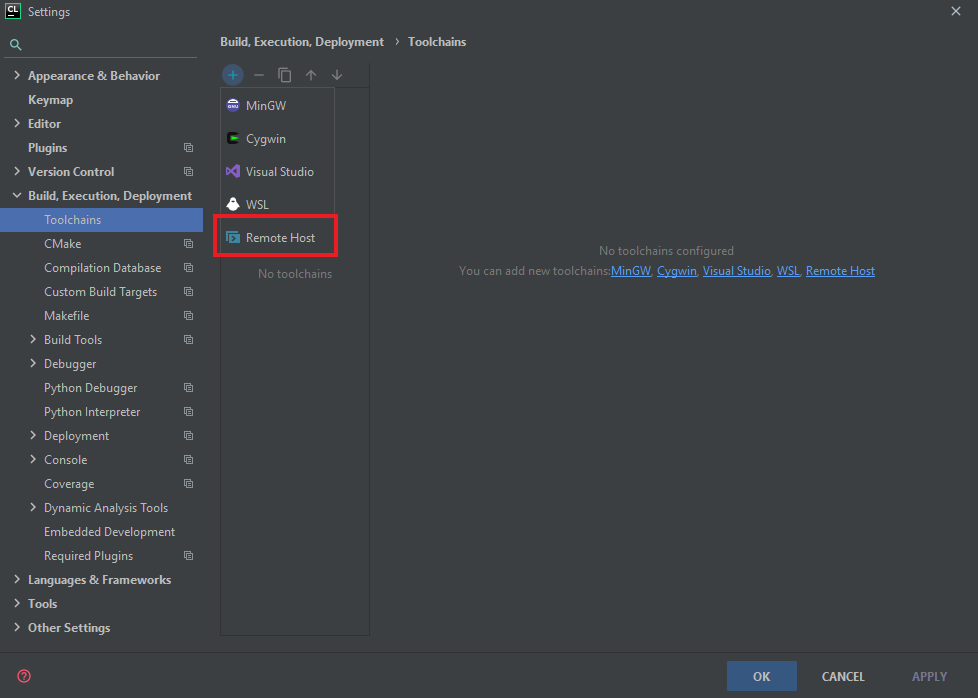
\includegraphics[width=0.5\textwidth]{images/beagleboneblack_truckcape_v4_images/CLionToolChainRemote.png}
                    \caption{CLion Remote Toolchain Option}
                    \label{fig:CLionToolChainRemote}
                \end{figure}
                \item Add new device credentials using the three dots to the right of the credentials field. (Fig. \ref{fig:CLionToolChainCredentialsButton}).
                \begin{figure}[H]
                    \centering
                    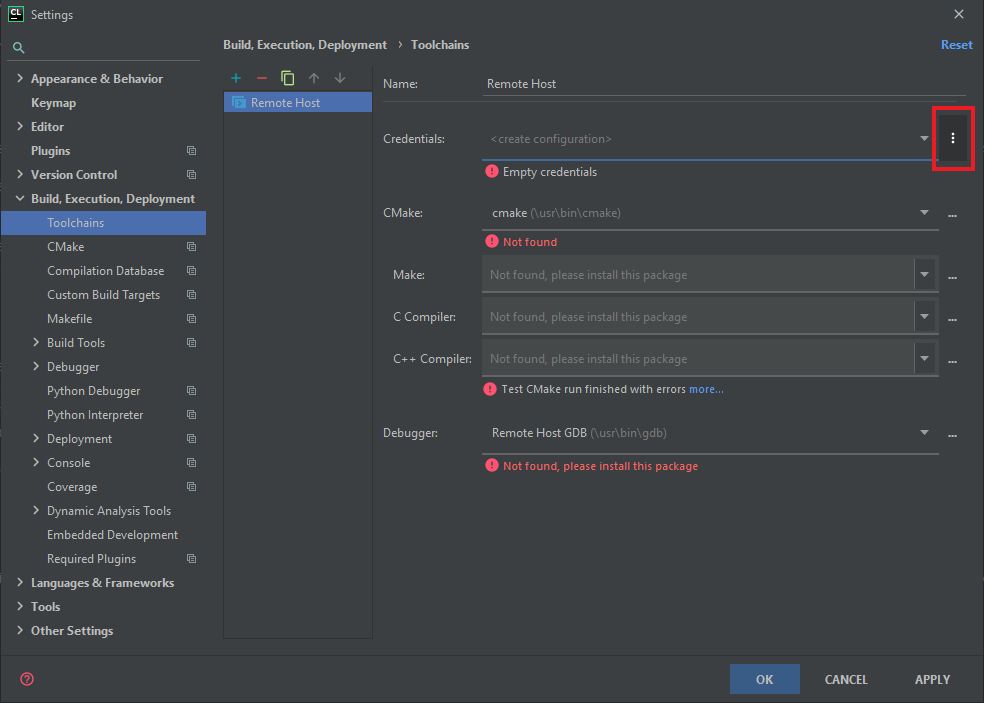
\includegraphics[width=0.5\textwidth]{images/beagleboneblack_truckcape_v4_images/ClionToolChainCredentialsButton.png}
                    \caption{CLion Remote Toolchain Credentials Button}
                    \label{fig:CLionToolChainCredentialsButton}
                \end{figure}
                \item Add device credentials just like PuTTY (Fig. \ref{fig:CLionToolChainCredentialsScreen}).
                \begin{figure}[H]
                    \centering
                    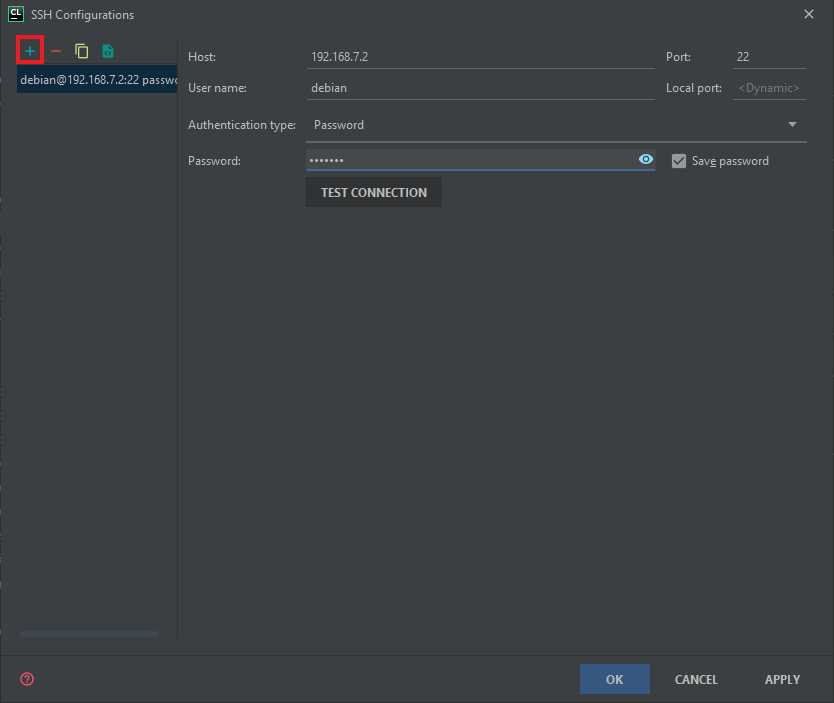
\includegraphics[width=0.5\textwidth]{images/beagleboneblack_truckcape_v4_images/ClionToolChainCredentialsScreen.png}
                    \caption{CLion Remote Toolchain Credentials Screen}
                    \label{fig:CLionToolChainCredentialsScreen}
                \end{figure}
                \item Test connection with the "Test Connection" button. If successful, click "Apply" then "OK."
                \item Now back on the Toolchains page, the credential field should say "Connected." However, the other fields may show errors. CMake as well as the C compiler must be installed on the beaglebone
                \begin{enumerate}
                    \item Connect to the BeagleBone using PuTTY. To install these packages, the BeagleBone should be connected to the internet. Although there are offline methods of installation, this guide will assume the BeagleBone is connected to the internet.
                    \item For installing CMake and GNU DeBugger (gdb), run the following commands:
                        \begin{lstlisting}[language=bash, autogobble=true]
                            $ sudo apt-get update -y
                            $ sudo apt-get update
                            $ sudo apt-get install cmake -y
                            $ sudo apt-get install gdb -y
                        \end{lstlisting}
                    \end{enumerate}
                \item Assuming the previous installation steps were successful, the Toolchain menu should now be connected to the BeagleBone and recognize that cmake and Remote Host GDB are installed. Click "Apply" and then "OK".
            \end{enumerate}
        \subsubsection{C Cross Compiling in Atom}
        \subsubsection{C Cross Compiling in Sublime Text}
        \subsubsection{C Cross Compiling in Visual Studio Code}
    \subsection{Remote Python Environment}
    The BeagleBone is configured with both Python 2 and Python 3. Text editors like Nano, VIM, and Emacs may be installed and used for writing Python scripts. However, the user may prefer to write scripts on an external device like a laptop. This portion of the guide covers Remote Python Development
        \subsubsection{Remote Python Environment using Jupyter Notebook}
        \subsubsection{Remote Python Environment for PyCharm}
        PyCharm Professional is required for configuring Remote Python Interpreters. This feature is not currently supported for PyCharm Community Edition. Like CLion, JetBrains offers free educational licenses for PyCharm Professional. 
        \begin{enumerate}
            \item Navigate to File, Settings, Project:, then "Python Interpreter."
            \item Select the button with three dots at the top right side of the screen (Fig. \ref{fig:PyCharmAddInterpreter}). Choose "Add..."
            \begin{figure}[H]
                \centering
                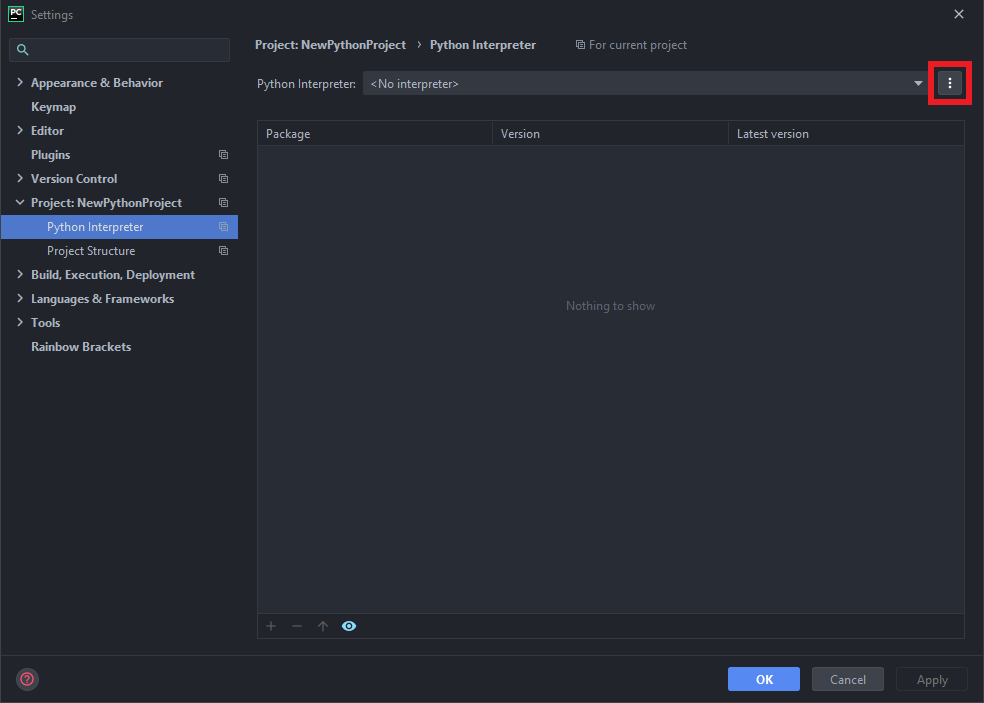
\includegraphics[width=0.5\textwidth]{images/beagleboneblack_truckcape_v4_images/PyCharmInterpreter.png}
                \caption{Add Interpreter to PyCharm}
                \label{fig:PyCharmAddInterpreter}
            \end{figure}
            \item Select "SSH Interpreter"
            \item Enter credentials just like other SSH utilities in the guide (Fig. \ref{fig:PyCharmSSHInterpreter})
            \begin{figure}[H]
                \centering
                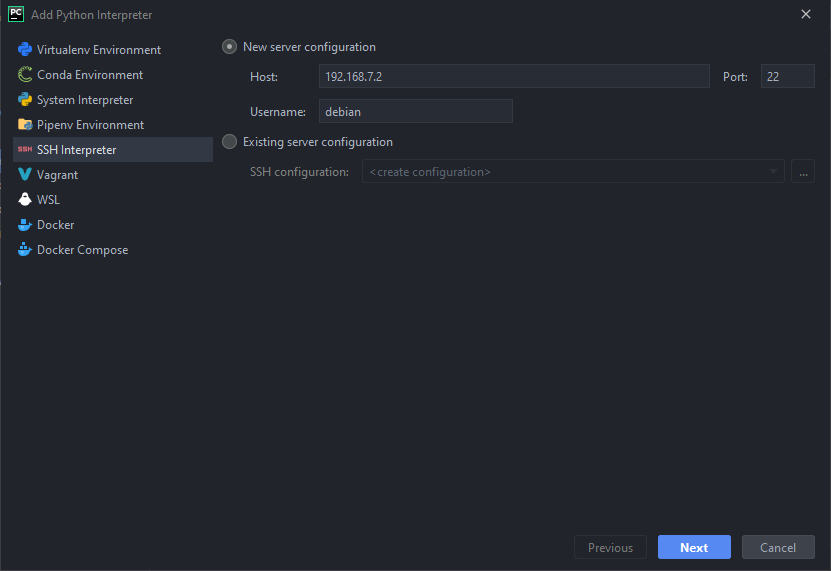
\includegraphics[width=0.5\textwidth]{images/beagleboneblack_truckcape_v4_images/PycharmSSHInterpreterCredentials.png}
                \caption{PyCharm SSH Credentials}
                \label{fig:PyCharmSSHInterpreter}
            \end{figure}
            \item Continue the setup pages, entering credentials when necessary.
            \item Choose where you want PyCharm to place files and which BeagleBone Python Interpreter to use.
            \item Once the setup pages have finished, select "Apply" and then "OK"
            \item The current PyCharm Project should now be configured to use the BeagleBone Python Interpreter.
        \end{enumerate}
        \subsubsection{Remote Python Environment for Atom}
        \subsubsection{Remote Python Environment for Sublime Text}
        \subsubsection{Remote Python Environment for Visual Studio Code}

\section{Programmable Realtime Units (PRU)}